 
\documentclass[a4paper,12pt]{article} % This defines  
\usepackage[top = 2.5cm, bottom = 2.5cm, left = 2.5cm, right = 2.5cm]{geometry} 

 
\usepackage[T1]{fontenc}
\usepackage[utf8]{inputenc}

\usepackage{graphicx} 
\usepackage[backend=biber,sorting=none, style=ieee]{biblatex}
\addbibresource{refe/referencia.bib}
\usepackage{setspace}
\setlength{\parindent}{0in}
\usepackage{wrapfig}

\usepackage{float}
 
\usepackage{fancyhdr}
\usepackage[breaklinks=true]{hyperref}

 \pagestyle{fancy}  

\fancyhf{} 

\lhead{\footnotesize} 

%\rhead works just like \lhead (you can also use \chead)
\rhead{\footnotesize Nuria Codesido Iglesias } %<---- Rellenar
 
\cfoot{\footnotesize \thepage} 

 \begin{document}

 \thispagestyle{empty}  

\begin{tabular}{p{15.5cm}}  
{\large \bf Hacking ético e Test de intrusión} \\ Máster Inter-Universitario en Ciberseguridad (MUNICS)  
 \\  Universidade da Coruña (UDC) y Universidade de Vigo (UVigo)\\ Curso 2024-2025  \\
\hline    
\\
\end{tabular}  
\vspace*{0.3cm}  

\begin{center}  
	{\Large \bf Práctica 1 - Descubrimiento y enumeración 
} % <---- Don't forget to put in the right number
	\vspace{2mm}
	
        % YOUR NAMES GO HERE
	{\bf Nuria Codesido Iglesias} % 
		
\end{center}  

\vspace{0.4cm}


%%%%%%%%%%%%%%%%%%%%%%%%%%%%%%%%%%%%%%%%%%%%%%%%
\section{Realiza un barrido ping (ICMP) sobre las máquinas proporcionadas. Captura con wireshark e identifica los cuatro paquetes esenciales del barrido}
\\
    El objetivo de este apartado es identificar qué máquinas están activas en la red mediante ICMP. Para ello, se utiliza la opción \textit{\texttt{-sn}} para detectar únicamente los hosts que están activos en la red sin realizar un escaneo de puertos de manera menos intrusiva (sin generar más tráfico del necesario). Cabe destacar que se utiliza la opción \textit{\texttt{--disable-arp-ping}} para forzar el uso de ICMP y cambiar el comportamiento del escaneo. Esto se debe a que cuando se realiza un escaneo en una red local (LAN), nmap suele priorizar ARP en vez de ICMP, ya que ARP es más confiable en estas redes. Finalmente, una vez que el escaneo se ha realizado, se guarda la salida en un fichero para poder procesar los resultados más tarde con herramientas como \textit{grep}. El comando utilizado: 
    \begin{center}
    \texttt{nmap -sn - -disable-arp-ping 192.168.56.0/24 -oG ejercicio1\_icmp.txt}
    \end{center}

    En esta primera imagen se visualiza la salida del comando anterior. El resultado nos indica que se escanearon 256 direcciones IP en la red 192.168.56.0/24 y encontraron 3 hosts activos: 192.168.56.6 (windows), 192.168.56.9 (linux) y 192.168.56.100 (máquina kali). Finalmente, se realiza un cat del fichero creado, para visualizar su contenido.
    
        \begin{figure} [hp!]
         \centering
         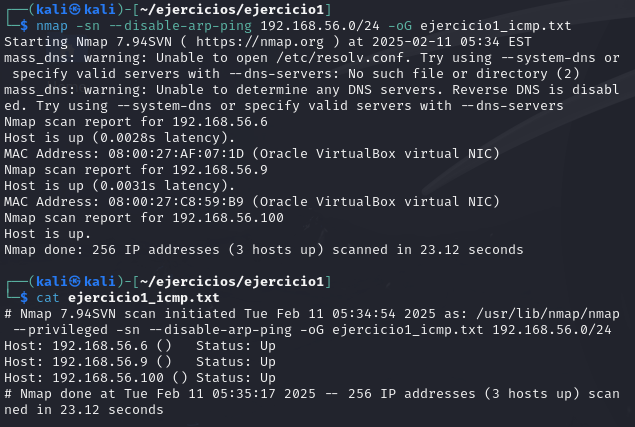
\includegraphics[width=0.6\textwidth]{Imagenes/nmap.png}
         \caption{Escaneo ping}
         \label{fig:nmapD}
        \end{figure}

        \newpage
        Por otro lado, al mismo tiempo se captura el tráfico con la herramienta Wireshark. Se observan paquetes ICMP y ARP:
            \begin{itemize}
                \item \textbf{\textit{Solicitud ICMP Echo Request (Ping Request).}}  Se visualizan paquetes ICMP enviados desde 192.168.56.100 (origen) hacia otras IPs en la red, como 192.168.56.9 y 192.168.56.6. Para verificar que máquinas están activas. (descubrimiento de hosts) \ref{fig:wire1}
                \item \textbf{\textit{Respuesta ICMP Echo Reply (Ping Reply). }} Algunos hosts (192.168.56.9, 192.168.56.6) responden a la solicitud, confirmando que están activos en la red. \ref{fig:wire1}
                \item \textbf{\textit{ARP Request (Broadcast.)}} La máquina 192.168.56.100 (origen) está intentando descubrir las direcciones MAC asociadas a las IPs de la red. A pesar, de haber utilizado la opción \textit{\texttt{--disable-arp-ping}}, es necesario para poder comunicarse con los hosts antes de enviar paquetes ICMP. \ref{fig:wire1}
                \item \textbf{\textit{ICMP Timestamp Request.}} Se usa para sincronizar la hora entre dispositivos de una red. \ref{fig:wire2}
            \end{itemize}
        \begin{figure} [hp!]
         \centering
         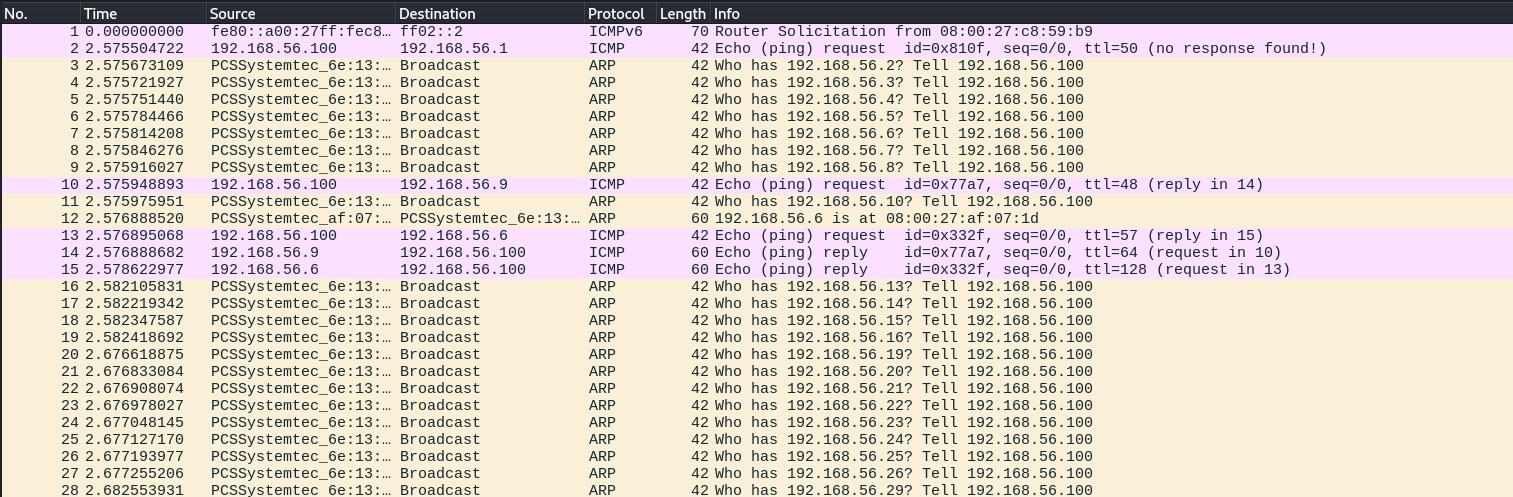
\includegraphics[width=1\textwidth]{Imagenes/wireshark-eje1.png}
         \caption{Wireshark}
         \label{fig:wire1}
        \end{figure}
        Entre todos estos paquetes, los cuatro paquetes esenciales son los ICMP Echo Request y Reply de las máquinas: 192.168.56.9 (rojo) y la 192.168.56.6 (azul). 
        \begin{figure} [hp!]
         \centering
         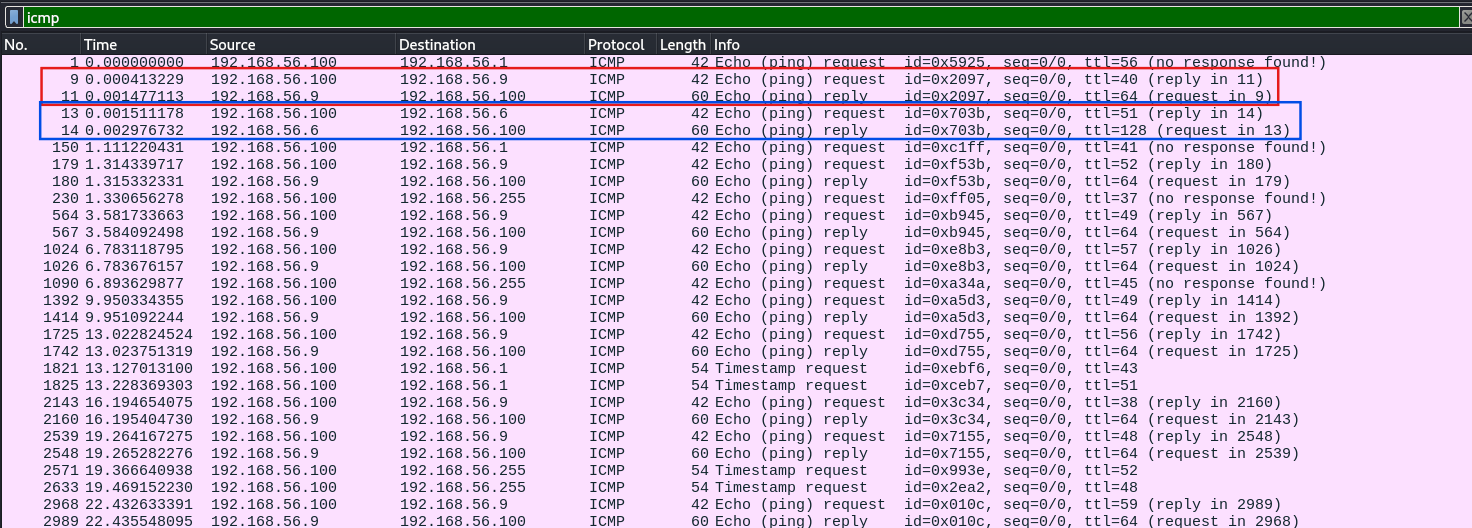
\includegraphics[width=1\textwidth]{Imagenes/icmp.png}
         \caption{Wireshark}
         \label{fig:wire2}
        \end{figure}



\\ \\
\section{Llevar a cabo un escaneo sigiloso (Stealth) de toda la red virtualizada. Comprobar el tráfico producido con Wireshark.}

El objetivo del escaneo sigiloso  implica un enfoque más discreto para detectar los servicios disponibles en una red sin ser fácilmente identificado. Por lo que a la hora de elegir los puertos que se van a escanear, se seleccionan los que corresponden a servicios clave. Para ello, se utiliza la opción \texttt{-p} para especificar los puertos que se quieren escanear, ya que si no se usa, \texttt{Nmap} escanea los 1000 puertos más comunes, lo que puede ser ruidoso y detectable. Los puertos seleccionados son:
\begin{itemize}
    \item 3389 (Windows) - Si este puerto está abierto, significa que se puede conectar a la máquina Windows usando Remote Desktop Protocol (RDP), lo que permite controlarla de manera remota. 
    \item 135 (Windows) - Se usa para iniciar conexiones RPC (Remote Procedure Call) con el servicio RPC Endpoint Mapper en sistemas Windows. Este servicio ayuda a asignar dinámicamente puertos para otros servicios que usan RPC.
    \item 139 (Windows) - Se usa para compartir archivos e impresoras.
    \item 22, 23 - Permite acceso remoto. 
    \item 21 -  Protocolo de transferencia de archivos, sin cifrado por defecto.
    \item 512,513,514 (Linux) - Usados para servicios de acceso remoto y ejecución de comandos.
    \item 80 - Puerto estándar para tráfico web sin cifrado.
    \item 443 - Puerto estándar para tráfico web cifrado con SSL/TLS.
    \item 49154, 49156 (Windows) - Puertos efímeros usados por Windows para RPC, SMB o conexiones internas.
    \item 3306 (MySQL), 5432 (PostgreSQL) -  Si estos puertos están abiertos, la máquina podría tener bases de datos activas.
    \item 5900 - Utilizado para control remoto de escritorio.
    \item 6000 (Linux) - Interfaz gráfica remota, si está abierto, se podrían espiar sesiones gráficas. 

\end{itemize}

    Por otro lado, también se utilizan más opciones de Nmap para hacerlo más discreto. La opción \texttt{-sS} realiza un escaneo "sigiloso" enviando paquetes sin establecer una conexión completa, lo que ayuda a evitar ser detectado. \texttt{-Pn} evita que \texttt{Nmap} envíe paquetes \texttt{ICMP} para verificar si los hosts están activos. Esto evita que el escaneo sea detectado por sistemas de monitoreo. Al usar esta opción se escanean todos los hosts, independientemente de si responden a los pings o no. Por último, \texttt{-n} evita que \texttt{Nmap} realice búsquedas \texttt{DNS} de las direcciones IP, lo que ayuda a prevenir que se genere tráfico visible en los registros de los servidores \texttt{DNS}. Cabe destacar que también se utiliza la opción \texttt{-oG} para guardar los resultados.
    
    \begin{center}
    \texttt{nmap -sS -n -Pn 192.168.56.0/24 -p 21,22,23,80,443,135,139,3389,49154,49156,3306,5432,5900,6000,512,513,514 -oG ejercicio2\_sigiloso.txt}
    \end{center}

    Una vez realizado el siguiente comando, se puede visualizar que puertos están activos en cada una de las máquinas. En las siguientes imágenes, se pueden observar que puertos están abiertos, filtrados o cerrados. 

        \begin{figure} [hp!]
         \centering
         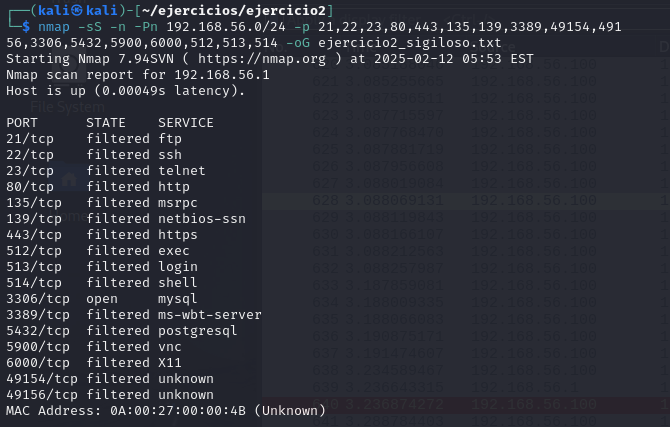
\includegraphics[width=0.5\textwidth]{Imagenes/silencioso1.png}
         \caption{Escaneo silencioso - 192.168.56.1 (gateway)}
         \label{fig:wireshark2}
        \end{figure}

        \begin{figure} [hp!]
         \centering
         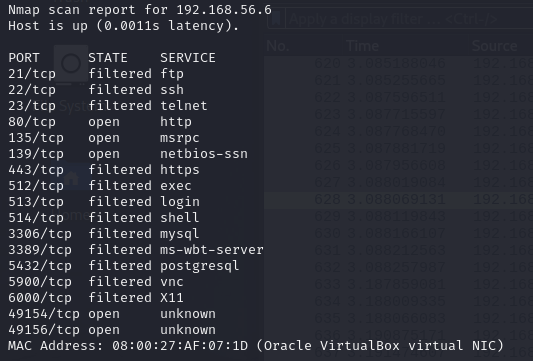
\includegraphics[width=0.5\textwidth]{Imagenes/sil2.png}
         \caption{Escaneo silencioso - 192.168.56.6 (Windows)}
         \label{fig:wireshark2}
        \end{figure}
        
\newpage
        \begin{figure} [hp!]
         \centering
         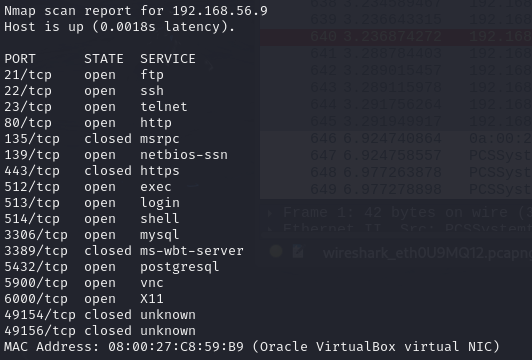
\includegraphics[width=0.5\textwidth]{Imagenes/sil3.png}
         \caption{Escaneo silencioso - 192.168.56.9 (Linux)}
         \label{fig:wireshark2}
        \end{figure}
        
        \begin{figure} [hp!]
         \centering
         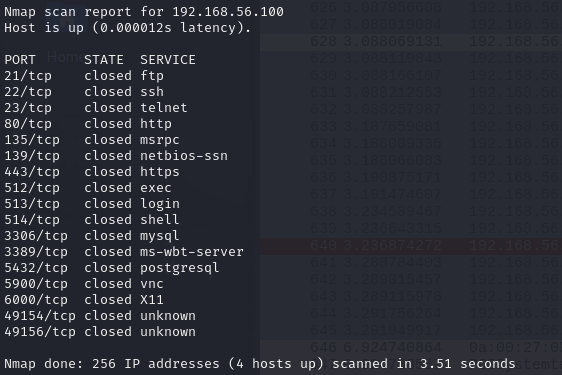
\includegraphics[width=0.5\textwidth]{Imagenes/sil4.png}
         \caption{Escaneo silencioso - 192.168.56.100 (kali)}
         \label{fig:wireshark2}
        \end{figure}

    Al ejecutar el comando, Wireshark captura el tráfico. Primero, se capturan los paquetes ARP broadcast porque el tráfico TCP funciona a nivel de capa 2 y necesita la dirección MAC para enviar los paquetes correctamente. Luego, Nmap envía paquetes TCP con el flag \texttt{SYN} para intentar iniciar la conexión con los puertos especificados. 
    \\\\
    La respuesta puede variar dependiendo de si el puerto está abierto, cerrado o filtrado. Si un puerto está abierto, una vez establecida la conexión (\texttt{SYN+ACK)}, en lugar de enviar un \texttt{ACK} para completar la conexión, Nmap envía un paquete \texttt{RST} para interrumpir la conexión. Esto no establece una conexión completa, simplemente permite verificar si el puerto está abierto sin completar el proceso de conexión. Con el fin de evitar la detección del escaneo por parte de firewalls o sistemas de intrusión. Un ejemplo (puerto 22 - máquina 192.168.56.9): en la imagen se visualiza en color azul, se verán 3 paquetes (\texttt{SYN, SYN+ACK, RST}).
    \\\\
    Por otro lado, si el puerto está cerrado, la máquina de destino responderá con un paquete \texttt{RST+ACK}. Un ejemplo (puerto 3389 - máquina 192.169.56.9): en la imagen, se visualiza en color rosa, se verán 2 paquetes (\texttt{SYN, RST+ACK}). Y si el puerto está filtrado el dispositivo no responderá. Un ejemplo (puerto 22 - máquina 192.168.56.1): en la imagen, se visualiza en color verde, se verá solo un paquete (\texttt{SYN}).
\newpage
        \begin{figure} [hp!]
         \centering
         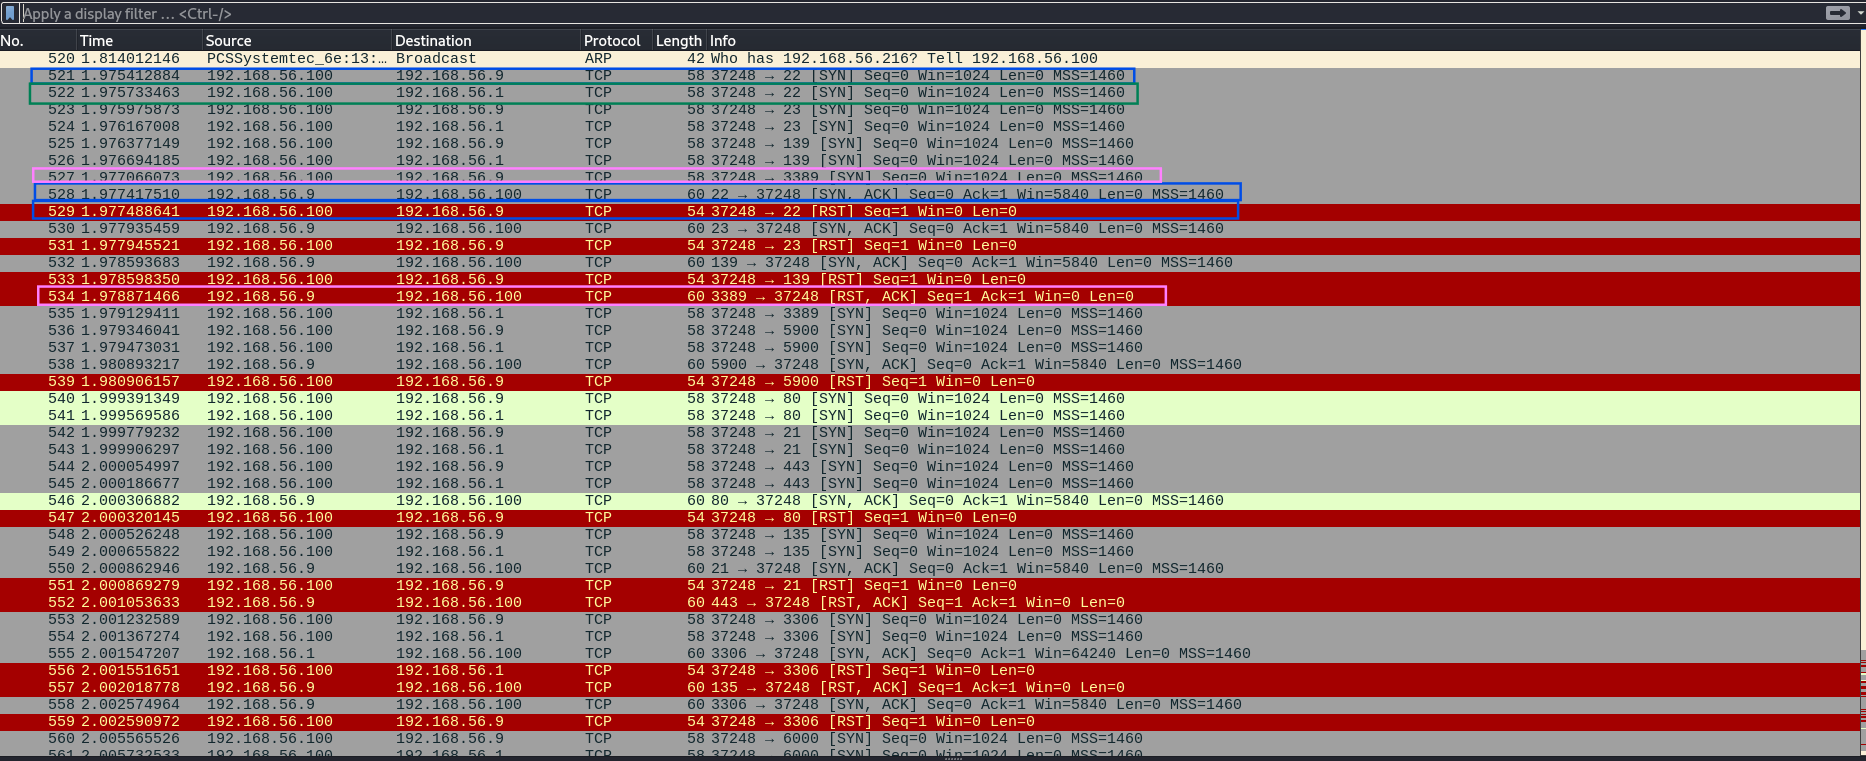
\includegraphics[width=1\textwidth]{Imagenes/wiresil.png}
         \caption{Wireshark - escaneo silencioso}
         \label{fig:wireshark2}
        \end{figure}





\\ \\
\section{Realizar un escaneo agresivo sobre una máquina de internet (por ejemplo http://scanme.nmap.org) y sobre alguna de la red virtualizada. Ayudarse de otras herramientas como Wireshark o la opción \textit{--packet-trace} de Nmap para comprobar similitudes y diferencias. }

Para este apartado, se tiene como objetivo realizar un escaneo agresivo, que busca recopilar la mayor cantidad de información posible mediante técnicas avanzadas que pueden ser más ruidosas y detectables. Para este escaneo, se utiliza la opción \texttt{-T4} para realizar un escaneo más rápido y agresivo. La opción \texttt{-A} para obtener más información, ya que utiliza funciones avanzadas como: detección del sistema operativo, la identificación de versiones de servicios, el uso de scripts para obtener más información y el traceroute para mapear la ruta hacia el objetivo. Finalmente, la opción \texttt{- -packet-trace}, como indica el enunciado, se emplea para ver un registro detallado de los paquetes enviados y recibidos durante el escaneo.

\paragraph{Escaneo agresivo - máquina de internet}
El primer comando utilizado es un escaneo agresivo a la máquina de internet (\texttt{scanme.nmap.org} - 45.33.32.156): 

    \begin{center}
    \texttt{nmap -A -T4 - -packet-trace  scanme.nmap.org -oG ejercicio3\_maquina.txt}
    \end{center}
    
Una vez se ejecuta el comando, al principio se realiza una exploración de puertos. Se visualizan los paquetes enviados \texttt{SENT}, que incluyen solicitudes ICMP para comprobar si la máquina (\texttt{scanme.nmap.org} - 45.33.32.156) está activa, así como solicitudes TCP para investigar los puertos abiertos. Además, se muestran las respuestas recibidas a esos paquetes RCVD. Esto se debe a que, al inicio de este escaneo agresivo, Nmap envía múltiples paquetes al destino para investigar puertos, servicios y otros detalles relacionados con la máquina de destino. También aparecen mensajes de depuración (trace) \texttt{NSOCK INFO}, que proporcionan información sobre el estado de los sockets que gestionan estas conexiones. Estos mensajes indican si las operaciones de escritura (SENT) y lectura (RCVD) en un socket fueron exitosas. 
\\

    En la imagen \ref{fig:ejer3Sent} se visualizan estos paquetes enviados. Se muestra un ejemplo de un paquete \texttt{SENT} (color rojo) TCP al puerto 80 enviado a la máquina destino (\texttt{scanme.nmap.org} - 45.33.32.156) y su respuesta \texttt{RVCD} (color azul). 
    
        \begin{figure} [hp!]
         \centering
         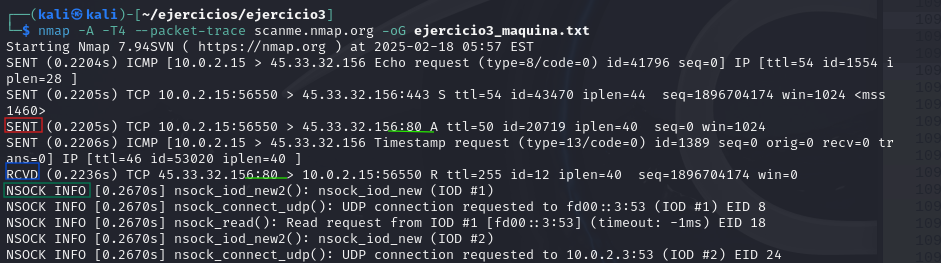
\includegraphics[width=1\textwidth]{Imagenes/ejer3_2SENT.png}
         \caption{Escaneo agresivo - máquina (\texttt{scanme.nmap.org} - 45.33.32.156) }
         \label{fig:ejer3Sent}
        \end{figure}

    Una vez realizada la fase de exploración de puertos, se interactúa con los diferentes servicios que tienen los puertos activos. En esta parte, empiezan a aparecer mensajes \texttt{NSE}. Que indica que Nmap está utilizando scripts NSE para interactuar con el servicio, para obtener información adicional y realizar un análisis más profundo. 
    \\
    Estos scripts pueden realizar diversas acciones, como establecer conexiones con puertos abiertos (\texttt{CONNECT}), enviar solicitudes para recopilar información sobre los servicios en ejecución, verificar configuraciones específicas...
\\ \\
    En la siguiente imagen \ref{fig:puerto80} se visualiza que se están realizando muchas conexiones repetidas a los puertos 80 y 22. 

\newpage
        \begin{figure} [hp!]
         \centering
         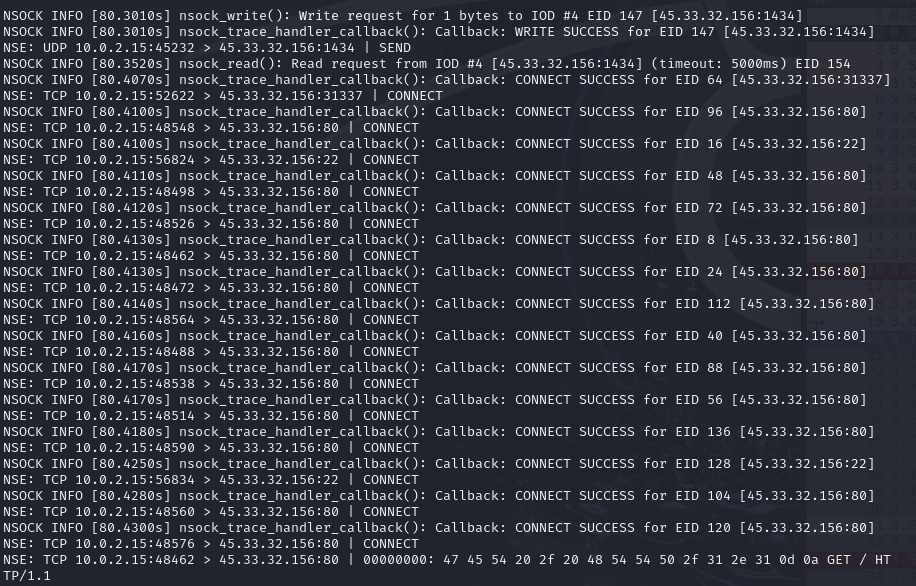
\includegraphics[width=0.8\textwidth]{Imagenes/puerto80Connect.png}
         \caption{Escaneo agresivo - máquina (\texttt{scanme.nmap.org} - 45.33.32.156) }
         \label{fig:puerto80}
        \end{figure}

    La siguiente imagen, es otro ejemplo de un mensaje, en el que se envía una petición HTTP al servidor \texttt{scanme.nmap.org} en el puerto 80. En este caso, se utiliza un script NSE para enviar una solicitud GET, que permite obtener detalles sobre la respuesta HTTP, como el código de estado (200 OK), los encabezados HTTP, el contenido de la página web, el servidor web utilizado (Apache), el sistema operativo que lo está ejecutando (Ubuntu) ...
    
    
        \begin{figure} [hp!]
         \centering
         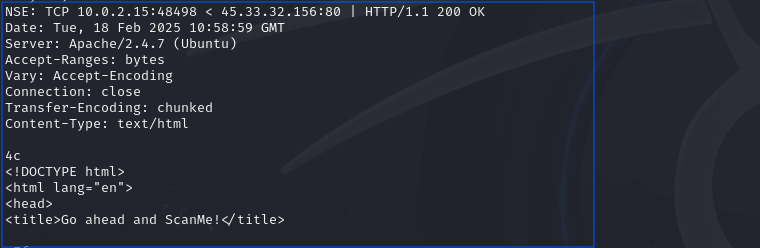
\includegraphics[width=0.8\textwidth]{Imagenes/NSESCANME.png}
         \caption{Escaneo agresivo - máquina (\texttt{scanme.nmap.org} - 45.33.32.156) }
         \label{fig:wireshark2}
        \end{figure}

    Por último, aparecen los puertos abiertos y sus servicios. Se encontraron cinco puertos abiertos y otros 995 cerrados.  A continuación, se proporciona información sobre la máquina \texttt{45.33.32.156}:
    \begin{itemize}
        \item \textbf{Tipo de dispositivo detectado.} En la imagen se visualiza en color verde.
        \item \textbf{Posible sistema operativo y virtualización: } Sugiere que el host está corriendo sobre un entorno virtualizado. En la imagen se visualiza en color azul.
        \item \textbf{Identificadores CPE: } El primero indica que podría ser un S.O. basado en VirtualBox. El segundo un sistema que está corriendo sobre QEMU (otro software de virtualización) y el tercero a un posible switch de Bay Networks. En la imagen se visualiza en color naranja.
        \item \textbf{Predicción agresiva del sistema operativo: }La detección agresiva de S.O. confirma que la mejor suposición de Nmap es que se trata de una máquina virtual en VirtualBox o QEMU. En la imagen se visualiza en color rosa.
        \item \textbf{Distancia de red: } La máquina está a solo 1 salto de distancia. Lo que indica que podría estar directamente accesible en Internet (sin firewalls intermedios). En la imagen se visualiza en color amarillo.
        \item \textbf{Información del S.O detectado: } Se detecta que el sistema operativo base es Linux. En la imagen se visualiza en color morado.
         \item \textbf{Tiempo de escaneo: } 86.36 segundos.
    \end{itemize}

        \begin{figure} [hp!]
         \centering
         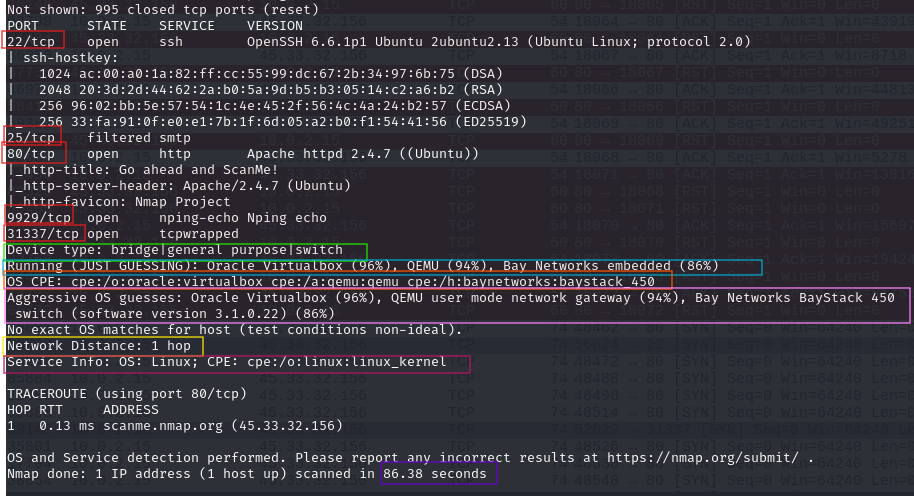
\includegraphics[width=1\textwidth]{Imagenes/infoSCANME.png}
         \caption{Escaneo agresivo - máquina (\texttt{scanme.nmap.org} - 45.33.32.156) }
         \label{fig:wireshark2}
        \end{figure}

\newpage
    Al mismo tiempo que se está ejecutando el comando, la herramienta Wireshark captura el tráfico, mostrando cada paquete en detalle. En la siguiente imagen se visualiza los primeros paquetes capturados.
        \begin{figure} [hp!]
         \centering
         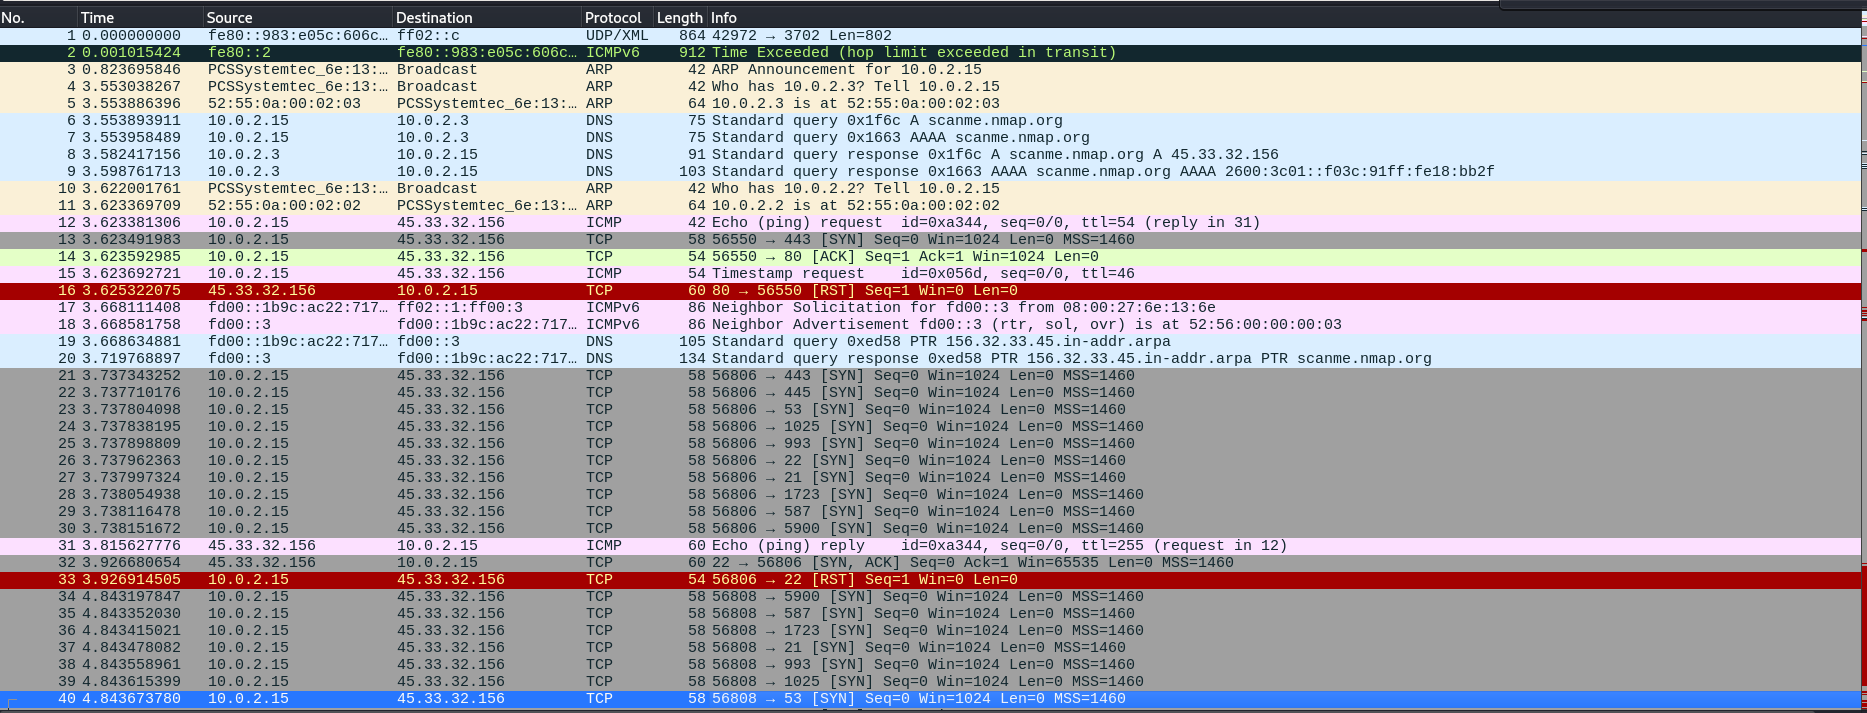
\includegraphics[width=1\textwidth]{Imagenes/wireMaquina.png}
         \caption{Wireshark - máquina (\texttt{scanme.nmap.org} - 45.33.32.156) }
         \label{fig:wireshark2}
        \end{figure}

\paragraph{Escaneo agresivo - red virtualizada }
 Para realizar este escaneo agresivo a una red virtualizada, se eligió la máquina 192.268.56.9 (Linux). Esta máquina se seleccionó porque tiene más puertos abiertos y menos puertos filtrados en comparación con la máquina de Windows.
        
    \begin{center}
    \texttt{nmap -A -T4  - -packet-trace  192.168.56.9 -oG ejercicio3\_red.txt}
    \end{center}

    Del mismo modo que en el escaneo a la máquina de internet, al ejecutar este comando, al principio se realiza una exploración de puertos. Se visualizan los paquetes enviados (\texttt{SENT}) y recibidos (\texttt{RCVD}), así como los mensajes de información \texttt{NSOCK INFO}.
    \\ \\
    En la imagen se representa en color rojo y azul, un paquete enviado (\texttt{SENT}) y su respuesta (\texttt{RCVD}) a un puerto abierto. Mientras que en color rosa y verde, un paquete enviado (\texttt{SENT}) a un puerto que no está abierto. La razón por la que se sabe que el puerto está cerrado es que, en este caso, el número de secuencia \texttt{seq} en la respuesta es igual a 0. 
\newpage
        \begin{figure} [hp!]
         \centering
         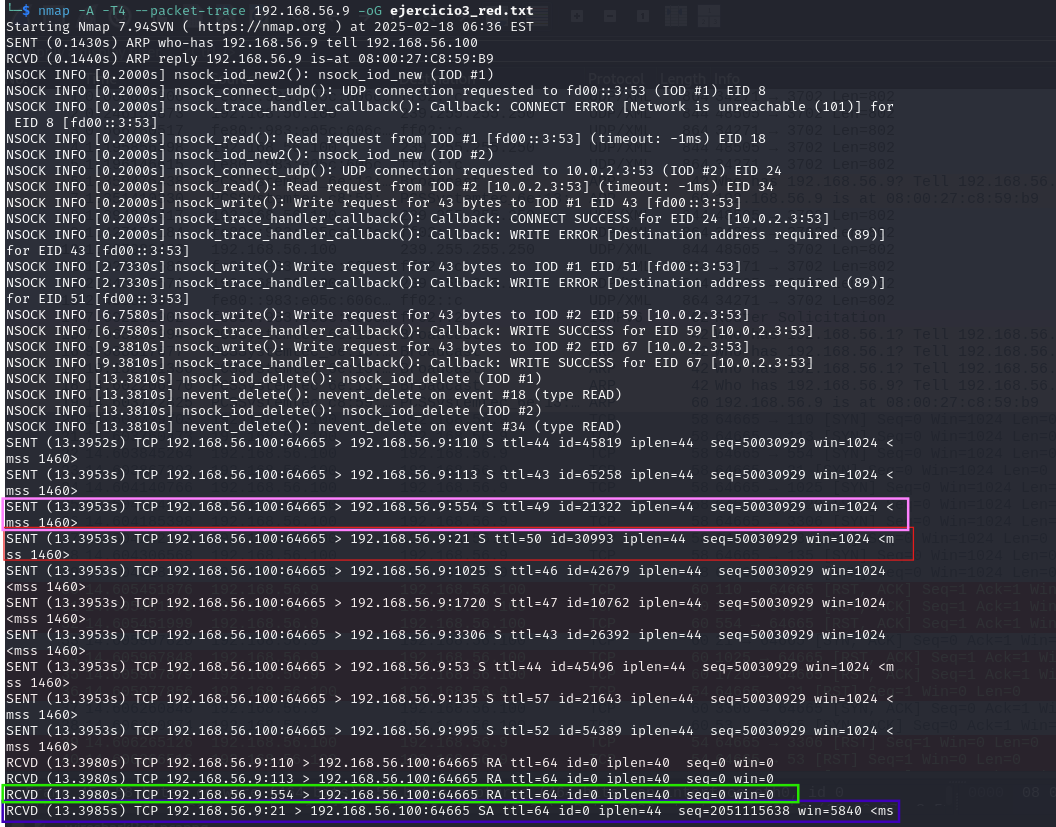
\includegraphics[width=1\textwidth]{Imagenes/sentred.png}
         \caption{Escaneo agresivo - máquina (192.168.56.9) }
         \label{fig:wireshark2}
        \end{figure}

    En este segundo escaneo, Nmap realiza un escaneo de servicios (\texttt{Service scan hard match}), enviando probes (sondeos) específicos para identificar el servicio que se está ejecutando en los puertos abiertos. En la siguiente imagen se visualiza un ejemplo (color azul). 
    \\ \\
    Cabe destacar que en la imagen, dentro del primer rectángulo de color rojo, se observa un mensaje de (\texttt{NSOCK INFO}) el cual indica que el puerto 1524 está proporcionando acceso a un shell remoto, como se evidencia en la respuesta (\texttt{root@metasploitable:/#}). Esto sugiere que dicho puerto está asociado a un servicio que permite la interacción directa con el sistema y que, en este caso, se ha obtenido acceso con privilegios de root. \\
    Por otro lado, en el segundo rectángulo, se confirma que el puerto 1524 tiene un bind shell, lo que significa que ofrece acceso remoto a un shell en la máquina sin necesidad de autenticación.
\newpage
        \begin{figure} [hp!]
         \centering
         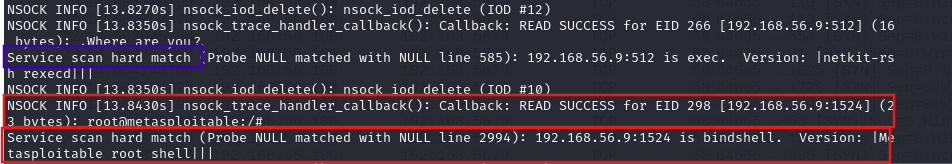
\includegraphics[width=1\textwidth]{Imagenes/servicescan.png}
         \caption{Escaneo agresivo - máquina (192.168.56.9) }
         \label{fig:wireshark2}
        \end{figure}

    En la siguiente imagen se visualiza como se puede tener acceso a esta máquina objetivo.
        \begin{figure} [hp!]
         \centering
         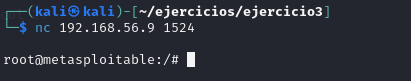
\includegraphics[width=0.8\textwidth]{Imagenes/acceso9.png}
         \caption{Acceso remoto - máquina (192.168.56.9) }
         \label{fig:wireshark2}
        \end{figure}
        
    Del mismo modo, también aparecen mensajes NSE asociados con los diferentes scripts NSE ejecutados. En la siguiente imagen, se visualiza un ejemplo en el que se realizó una conexión HTTP y su respuesta, que indica que el puerto 80 está corriendo Apache y sirviendo una página web de \texttt{Metasploitable2} (S.O.intencionalmente vulnerable).
    
        \begin{figure} [hp!]
         \centering
         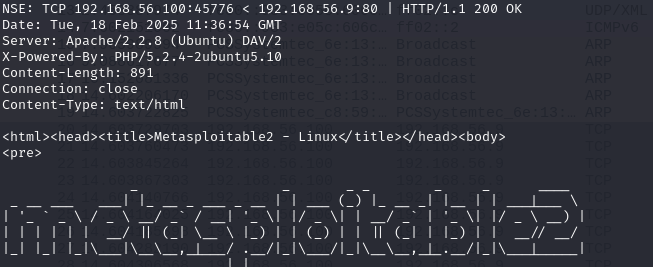
\includegraphics[width=0.8\textwidth]{Imagenes/meta.png}
         \caption{Acceso remoto - máquina (192.168.56.9) }
         \label{fig:wireshark2}
        \end{figure}

\newpage
   En la siguiente imagen \ref{fig:80diferente} se visualiza que se están realizando muchas conexiones repetidas a los puertos 137, 80, 8180, 5900, 1434, entre otros. En comparación con la máquina de Internet, que solo la mayoría de conexiones repetidas pertenece a los puertos 80 y 22, esto sugiere que la máquina de Linux pertenece a una red interna con una mayor cantidad de servicios y puertos accesibles. Esto puede indicar que no está protegida por un firewall tan restrictivo como el de la máquina en Internet, permitiendo el escaneo y la interacción con una variedad más amplia de servicios.

        \begin{figure} [hp!]
         \centering
         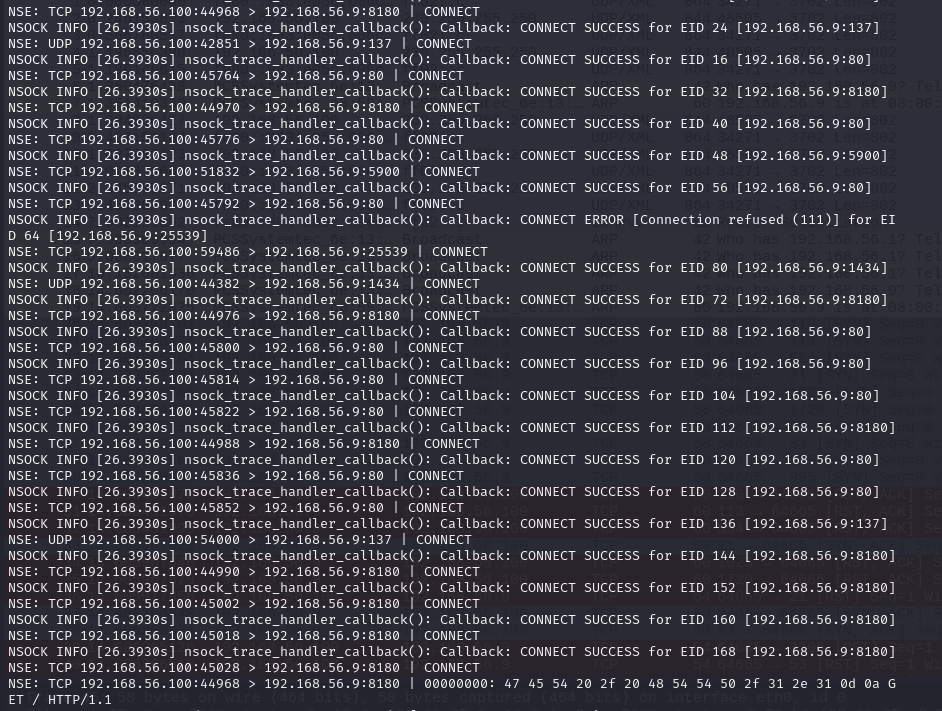
\includegraphics[width=0.8\textwidth]{Imagenes/puertosdiferentes80.png}
         \caption{Acceso remoto - máquina (192.168.56.9) }
         \label{fig:80diferente}
        \end{figure}
        
        Por último, aparecen los puertos abiertos (23) y sus servicios. A continuación, se proporciona información sobre la máquina 192.168.56.9:
    \begin{itemize}
        \item \textbf{Tipo de dispositivo detectado.} Se identifica como un dispositivo de propósito general, lo que significa que no es un dispositivo especializado, sino un sistema más general. En la imagen se visualiza en color verde.
        \item \textbf{Running: } Indica que la máquina está ejecutando Linux 2.6.X . En la imagen se visualiza en color verde oscuro.
        \item \textbf{Identificadores CPE: } Se refiere al kernel de Linux versión 2.6. En la imagen se visualiza en color naranja.
        \item \textbf{OS Details: }Se especifica que el sistema operativo es Linux 2.6.9 - 2.6.33. En la imagen se visualiza en color rosa.
        \item \textbf{Distancia: } La máquina está a solo 1 salto de distancia. Lo que indica que está directamente conectada a tu red sin intermediarios. En la imagen se visualiza en color amarillo.
        \item \textbf{Información del S.O detectado: } Los nombres de host asociados son \\ \texttt{metasploitable.localdomain} y \texttt{irc.Metasploitable.LAN}. Esto indica que la máquina está identificada en la red como metasploitable. Por otro lado, el sistema operativo identificado es Unix (Linux). En la imagen se visualiza en color morado.
        \item \textbf{Tiempo de escaneo:} 41.34 segundos.
    \end{itemize}
        
        \begin{figure} [hp!]
         \centering
         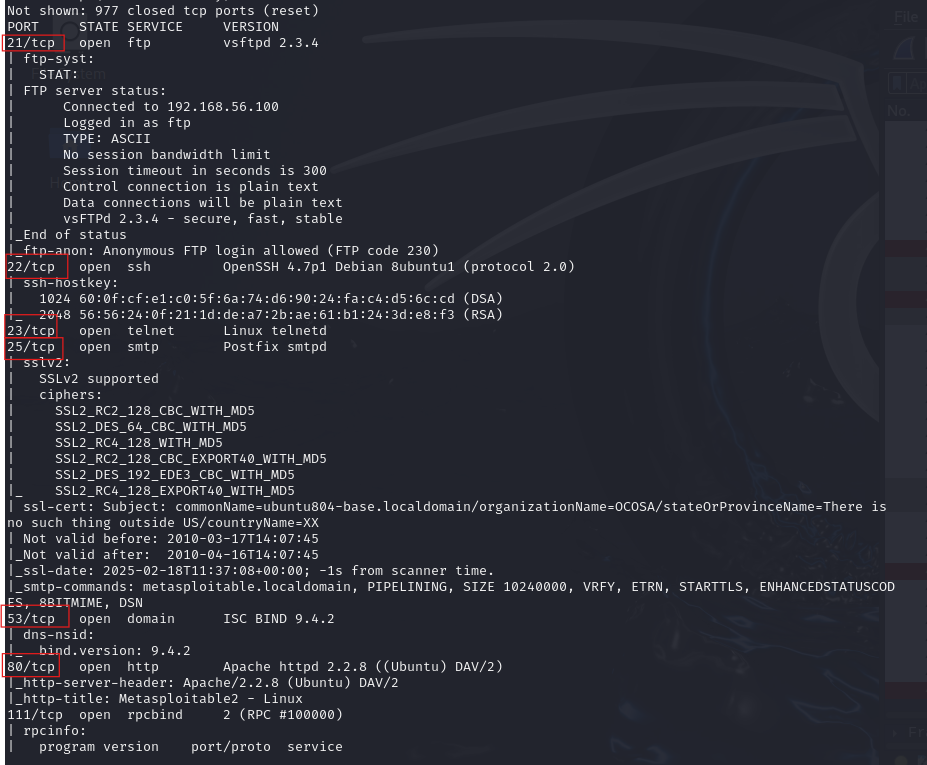
\includegraphics[width=0.8\textwidth]{Imagenes/puertos9.png}
         \caption{Acceso remoto - máquina (192.168.56.9) }
         \label{fig:wireshark2}
        \end{figure}
        
\newpage

        \begin{figure} [hp!]
         \centering
         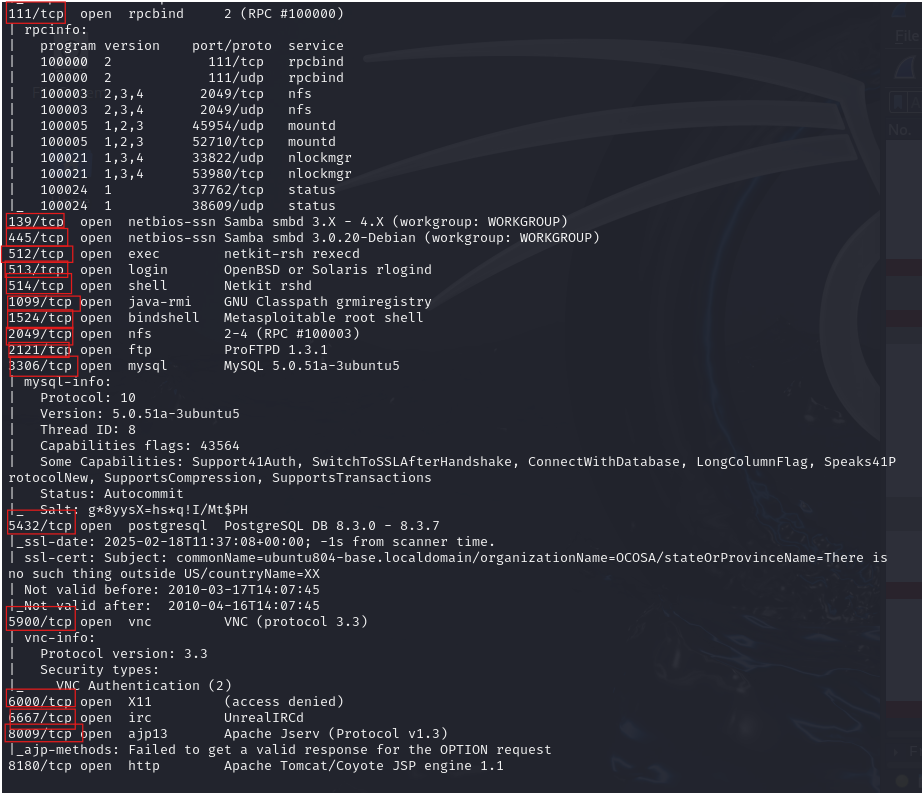
\includegraphics[width=0.8\textwidth]{Imagenes/puertos91 - copia.png}
         \caption{Acceso remoto - máquina (192.168.56.9) }
         \label{fig:wireshark2}
        \end{figure}

        \begin{figure} [hp!]
         \centering
         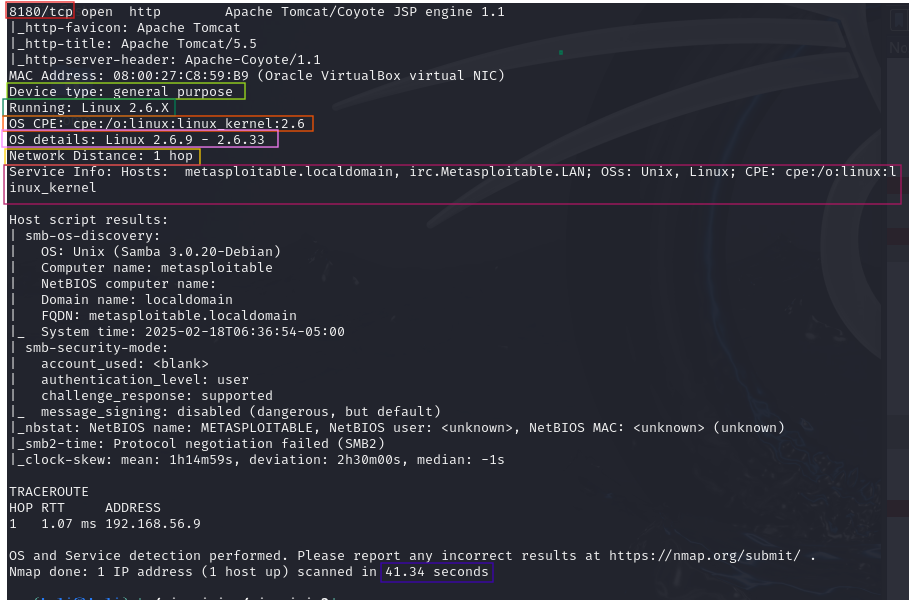
\includegraphics[width=0.8\textwidth]{Imagenes/info2.png}
         \caption{Acceso remoto - máquina (192.168.56.9) }
         \label{fig:wireshark2}
        \end{figure}

\newpage
    Mientras se ejecuta el comando, Wireshark está capturando el tráfico de red y mostrando cada paquete en detalle. En la imagen siguiente se pueden ver los primeros paquetes capturados durante el proceso.
 
        \begin{figure} [hp!]
         \centering
         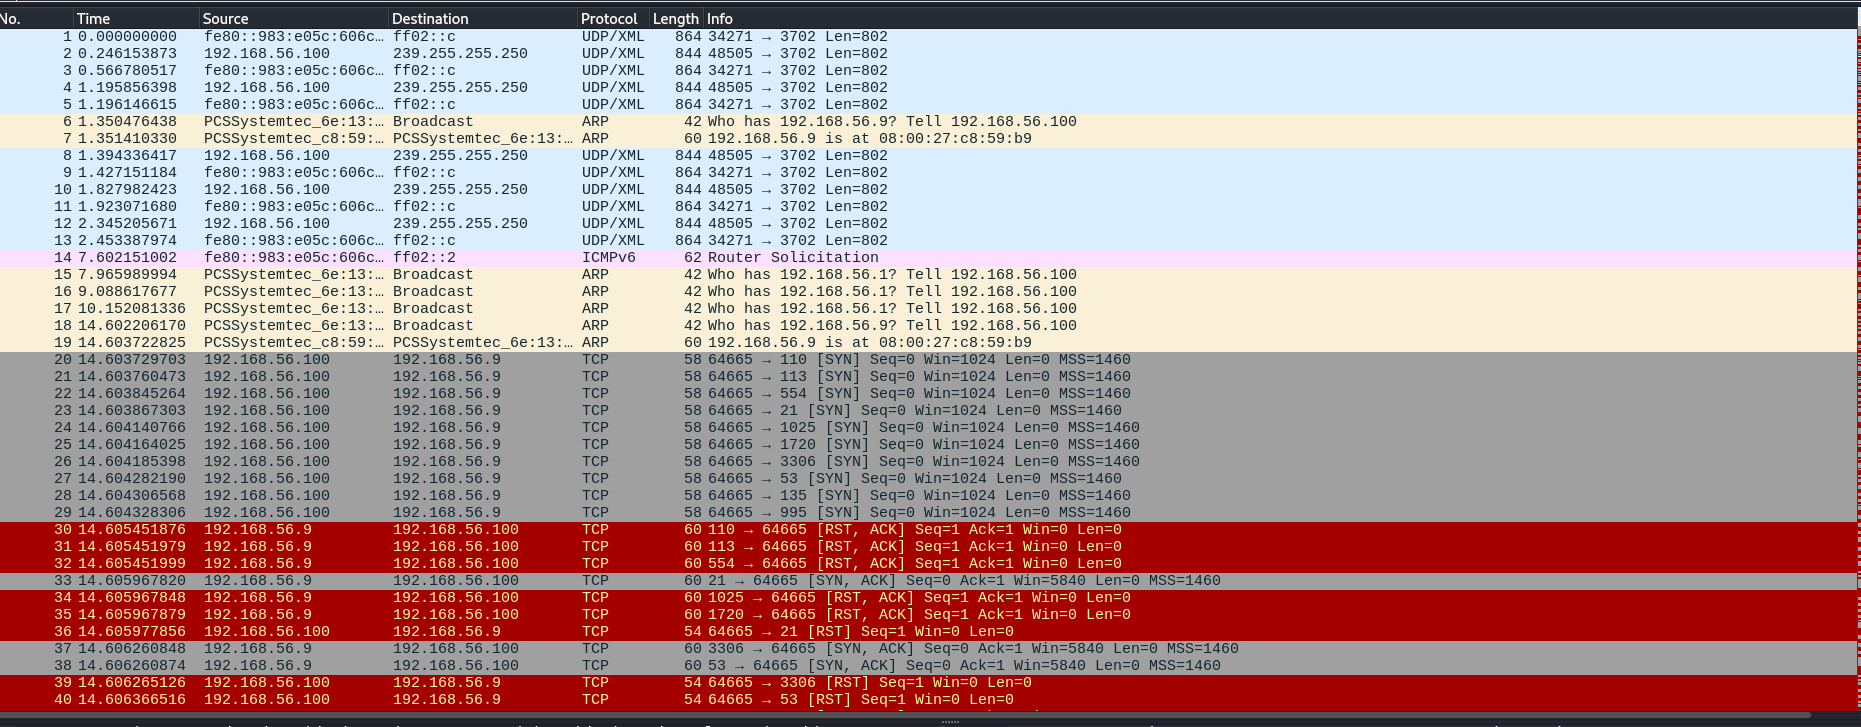
\includegraphics[width=1\textwidth]{Imagenes/wireRed.png}
         \caption{Wireshark - máquina (192.168.56.9) }
         \label{fig:wireshark2}
        \end{figure}

   
    \paragraph{Diferencias.}
    \begin{itemize}
        \item \textbf{Tiempo de escaneo: }La máquina de internet \texttt{scanme} tiene una menor velocidad (86.36 segundos), en relación a la máquina que se encuenta en la misma red (41.34 segundos). Esto se debe a factores como la mayor latencia de la red pública y la posible presencia de algún firewall que agregan retrasos en el proceso de escaneo.

        \item \textbf{Seguridad: } La máquina en Internet parece estar configurada con medidas de seguridad más estrictas, ya que solo tiene 5 puertos abiertos. En cambio, la máquina en la red local tiene 23 puertos abiertos, lo que indica una configuración de seguridad más débil y menos restricciones de acceso.

        \item \textbf{Wireshark: }En la máquina de Linux se observa una mayor cantidad de servicios disponibles y más tráfico debido a la mayor cantidad de puertos abiertos.

        \item \textbf{Paquete - Service scan hard match:} En la máquina Linux se registran paquetes de tipo \texttt{Service scan hard match}. Esto se debe a que Nmap tiene un acceso más directo a los servicios, debido a que la máquina tiene una configuración de red menos restrictiva en comparación con la máquina de Internet.
        
    \end{itemize}


\newpage

\\ \\
\section{Realizar un escaneo lo más rápido posible (insane) sobre las máquinas disponibles. Comprobar además la versión de los servicios implementados. Buscar al menos una vulnerabilidad en https://cve.mitre.org/ para cada uno de esos servicios.}

Para este apartado, se tiene como objetivo realizar un escaneo lo más rápido posible (insane). Para ello, se utiliza la opción \texttt{-T5}, que permite establecer el escaneo en el modo más rápido. Además, se emplea la opción \texttt{-sV} para detectar las versiones de los servicios que están corriendo en los puertos abiertos. 

    \paragraph{Escaneo insane - máquina 192.168.56.6}
    La primera máquina en la que se realiza el escaneo \texttt{insane} es la de Windows (\texttt{192.168.56.6}). El comando utilizado es:
    
    \begin{center}
    \texttt{nmap -sV -T5 192.168.56.6  -oG ejercicio4\_maquina6.txt}
    \end{center}

    En la siguiente imagen se visualizan los puertos abiertos, los servicios detectados y sus respectivas versiones tras el escaneo. 
    
        \begin{figure} [hp!]
         \centering
         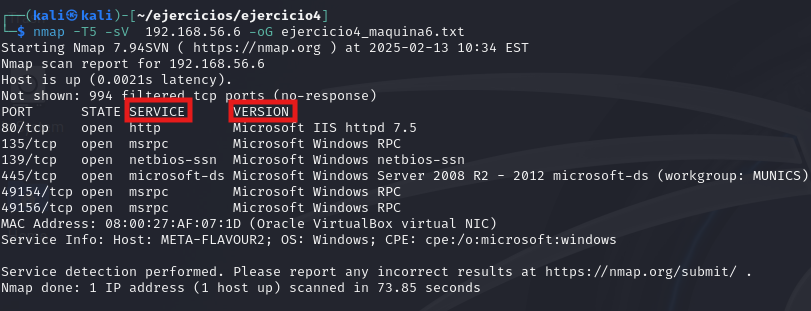
\includegraphics[width=1\textwidth]{Imagenes/vuln6.png}
         \caption{Escaneo insane - máquina (192.168.56.6) }
         \label{fig:wireshark2}
        \end{figure}

\begin{enumerate}
    \item  \textbf{Servicio - http:} En relación al servicio http con la versión \texttt{Microsoft IIS httpd 7.5}, se encontraron las vulnerabilidades \texttt{CVE-2010-2730}, \texttt{CVE-2010-3972} y \texttt{CVE-2010-1899}. 
    \begin{itemize}
        \item \textbf{CVE-2010-2730: } ~\cite{cve1} Esta vulnerabilidad es un desbordamiento de búfer que afecta a \texttt{Microsoft IIS 7.5} cuando FastCGI está habilitado, permitiendo a un atacante remoto ejecutar código arbitrario mediante el envío de encabezados de solicitud especialmente diseñados.
        \item \textbf{CVE-2010-3972: }  ~\cite{cve2} Esta vulnerabilidad es un desbordamiento de búfer que afecta a \texttt{Microsoft IIS 7.5}. Cuando un atacante envía solicitudes HTTP maliciosas al servidor IIS, se puede provocar una ejecución remota de código.
        \item \textbf{CVE-2010-1899: } ~\cite{cve3} Esta vulnerabilidad permite a un atacante realizar una elevación de privilegios en un sistema que ejecuta \texttt{Microsoft IIS 7.5}.
    \end{itemize}

    \item \textbf{Servicio - msrpc: } Se encontró la vulnerabilidad \texttt{CVE-2020-1113}  ~\cite{cve4}  en el servicio \texttt{Microsoft Remote Procedure Call}, la cual está relacionada con una falla en Windows RPC que permite la elevación de privilegios. 
    
    \item \textbf{Servicio - netbios-ssn: } En relación a este servicio se encontró la vulnerabilidad \texttt{CVE-2018-7445}  ~\cite{cve5}. Esta vulnerabilidad está asociada con un desbordamiento de búfer en el servicio \texttt{NETBIOS}, que es utilizado en redes Windows para compartir recursos y realizar comunicación entre sistemas.
    
    \item  \textbf{Servicio - microsoft-ds: } Se detectó una vulnerabilidad en el servicio Microsoft SMBv1 a través del puerto 445/tcp, en el servicio \textit{microsoft-ds}, que corresponde a la vulnerabilidad \texttt{CVE-2017-0143} ~\cite{cve6}. Esta vulnerabilidad afecta a varias versiones de Windows,  incluida la versión utilizada en el servidor  \texttt{Windows Server 2008 R2}. Este servicio contiene una debilidad crítica que permite a un atacante remoto ejecutar código arbitrario en el sistema afectado.

\end{enumerate}


        
   \paragraph{Escaneo insane - máquina 192.168.56.9}
    A continuación, se realiza el escaneo \texttt{insane} a la máquina de Linux (\texttt{192.168.56.9}). El comando utilizado es:

    \begin{center}
    \texttt{nmap -sV -T5 192.168.56.9  -oG ejercicio4\_maquina9.txt}
    \end{center}

        \begin{figure} [hp!]
         \centering
         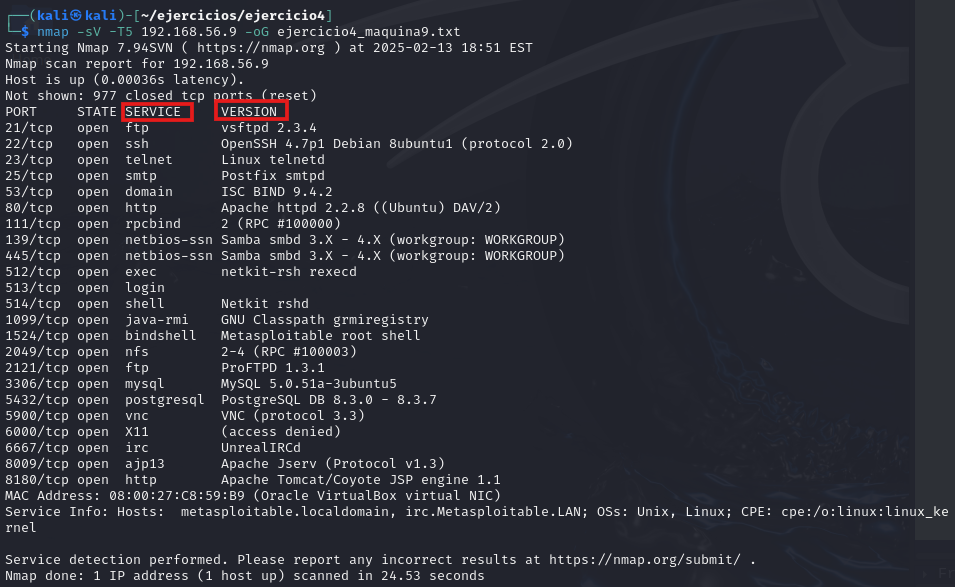
\includegraphics[width=1\textwidth]{Imagenes/insane9.png}
         \caption{Escaneo insane - máquina (192.168.56.9) }
         \label{fig:wireshark2}
        \end{figure}

    \begin{enumerate}
        \item \textbf{Servicio - ftp: }Para este servicio, se encontró la vulnerabilidad \texttt{CVE-2011-2523} ~\cite{cve7}, la cual afecta a \texttt{vsftpd 2.3.4}. Esta vulnerabilidad ocurre debido a la presencia de un backdoor en el código fuente comprometido del servidor FTP.
        \item \textbf{Servicio - ssh: } Se encontró la vulnerabilidad \texttt{CVE-2008-5161}  ~\cite{cve8}, la cual afecta a la versión \texttt{OpenSSH 4.7p1 Debian 8ubuntu1}. Esta vulnerabilidad en los modos CBC permite a un atacante recuperar partes de texto sin cifrar analizando la longitud de los paquetes SSH.
        \item \textbf{Servicio - telnet: } En relación a este servicio telnet, se encontró la vulnerabilidad \texttt{CVE-2005-2040}  ~\cite{cve9}, la cual es un desbordamiento de búfer en telnetd.
        \item \textbf{Servicio - smtp: } Para este servicio, se encontró la vulnerabilidad \texttt{CVE-2015-4000} ~\cite{cve10}. Esta vulnerabilidad afecta a Postfix smtpd y permite un ataque de denegación de servicio (DoS).
        \item \textbf{Servicio - domain: } Se encontró la vulnerabilidad \texttt{CVE-2008-0122} ~\cite{cve11}, la cual está relacionada con un problema de desbordamiento de búfer en el servicio de DNS de BIND.
        \item \textbf{Servicio - http: } Para este servicio, se encontró la vulnerabilidad \texttt{CVE-2017-3167} ~\cite{cve12}. Esta vulnerabilidad se relaciona con una falta de validación de las entradas de usuario en el módulo \textit{mod\_dav} de \texttt{Apache HTTPD}.
        \item \textbf{Servicio - rpcbind: } Se encontró la vulnerabilidad \texttt{CVE-2017-8779} ~\cite{cve13}, que permite causar una denegación de servicio (DoS) debido a una asignación incorrecta de memoria al enviar un paquete UDP malicioso al puerto 111.
        \item \textbf{Servicio - netbios-ssn: }  En relación con los servicios \textit{Samba smbd 3.X - 4.X} en los puertos 139/tcp y 445/tcp, se encontró la vulnerabilidad \texttt{CVE-2023-42670} ~\cite{cve14}.
        \item \textbf{Servicio - exec: } Se encontró la vulnerabilidad \texttt{CVE-1999-0651} ~\cite{cve15}, que afecta al servicio \texttt{netkit-rsh rexecd}. Esta vulnerabilidad es una debilidad en la autenticación del servicio rexecd, utilizado para ejecutar comandos de manera remota. De tal modo, que permite a un atacante ejecutar comandos arbitrarios.
        \item \textbf{Servicio - login: } Se encontró la vulnerabilidad \texttt{CVE-1999-0502} ~\cite{cve16}, la cual afecta al servicio \texttt{rexecd} en el puerto 513/tcp. Esta vulnerabilidad permite a los atacantes ejecutar comandos arbitrarios sin necesidad de autenticarse,
        \item \textbf{Servicio - shell: } Se detectó la vulnerabilidad \texttt{CVE-1999-1126} ~\cite{cve17}, que afecta al servicio \texttt{Netkit rshd} en el puerto 514/tcp. Esta vulnerabilidad se debe a un desbordamiento de búfer en el rshd, que permite la ejecución de código arbitrario. 
        \item \textbf{Servicio - java-rmi: } Se encontró la vulnerabilidad \texttt{CVE-2011-3556} ~\cite{cve18}, que afecta al servicio \texttt{GNU Classpath grmiregistry} en el puerto 1099/tcp. Esta vulnerabilidad permite la ejecución remota de código al manipular objetos RMI.
        \item \textbf{Servicio - bindshell: } No se encontró ninguna vulnerabilidad en \texttt{CVE List}.
        \item \textbf{Servicio - nfs: } No se encontró ninguna vulnerabilidad en \texttt{CVE List}.
        \item \textbf{Servicio - ftp: }El servicio FTP ProFTPD versión 1.3.1 está afectado por la vulnerabilidad \texttt{CVE-2009-0543} ~\cite{cve19}. Esta vulnerabilidad permite a los atacantes remotos ejecutar código SQL arbitrario en el sistema objetivo.
        \item \textbf{Servicio - mysql: } Se encontró la vulnerabilidad \texttt{CVE-2008-4097} ~\cite{cve20} que afecta a \texttt{MySQL 5.0.51a}. Esta vulnerabilidad permite a usuarios locales eludir verificaciones de privilegios mediante el uso de \texttt{symlinks} en tablas MyISAM.
        \item \textbf{Servicio - postgresql: } Se detectó la vulnerabilidad \texttt{CVE-2010-1447} ~\cite{cve21}, que permite a atacantes eludir restricciones de acceso en el módulo \texttt{Safe.pm} de \texttt{Perl}, ejecutando código arbitrario. 
        \item \textbf{Servicio - vnc: } En relación a este servicio, se encontró la vulnerabilidad \texttt{CVE-2002-1511} ~\cite{cve22} , que afecta a versiones anteriores a 3.3.3r2-21 debido al uso de rand() en lugar de srand(), lo que genera cookies débiles.
        \item \textbf{Servicio - x11: } No se encontró ninguna vulnerabilidad en \texttt{CVE List}.
        \item \textbf{Servicio - irc: } Se encontró la vulnerabilidad \texttt{CVE-2010-2075} ~\cite{cve23} . Esta vulnerabilidad afecta a \texttt{UnrealIRCd 3.2.8.1} debido a una modificación externa (Trojan Horse) en el macro \texttt{DEBUG3\_DOLOG\_SYSTEM}, esto permite ejecutar comandos arbitrarios de manera remota.
        \item \textbf{Servicio - ajp13: } Se encontró la vulnerabilidad \texttt{CVE-2020-1938} ~\cite{cve24}  que afecta al puerto 8009/tcp y al servicio \texttt{ajp} versión 1.3. Esta vulnerabilidad,  permite a los atacantes remotos leer archivos arbitrarios desde cualquier lugar de la aplicación web y procesar cualquier archivo como \texttt{JSP} (JavaServer Pages).
        \item \textbf{Servicio - http: } Se detectó la vulnerabilidad \texttt{CVE-2005-2090} ~\cite{cve25} , que afecta a la versión encontrada, \texttt{Apache Tomcat 5.0.19 (Coyote/1.1)}, permitiendo ataques de HTTP Request Smuggling.
    \end{enumerate}

\\ \\
\section{Describir las diferencias observadas en relación al descubrimiento de los equipos disponibles}
\\
A través de los escaneos realizados, se han identificado dos máquinas activas en la red virtualizada: máquina Windows (192.168.56.6) y máquina Linux (192.168.56.9).  A continuación se describen las principales diferencias observadas entre ambas máquinas:

\paragraph{Sistema operativo.}
La diferencia más significativa entre ambas máquinas es el sistema operativo. En el caso de la máquina 192.168.56.9 el S.O. identificado, es Linux 2.6.9-2.6.33. Mientras que la 192-168.56.6 es \texttt{Windows Server 2008 R2 Enterprise}. \\ \\
Además del sistema operativo, se observan diferencias en los nombres de host de las máquinas. El equipo 192.168.56.9 se identifica como \texttt{metasploitable} y el otro como \texttt{META-FLAVOUR2}.

\paragraph{Tiempo de respuesta.}
Otra diferencia es el tiempo de respuesta de cada máquina (latencia), se visualiza en la imagen \ref{fig:nmapD}. Windows tiene una latencia más baja (0.0028s) que Linux (0.0031s). 

\paragraph{Puertos.}
 En cuanto al escaneo de los puertos, se observan diferencias significativas en relación a sus estados. A la hora de realizar un escaneo stealth de los servicios clave, en la máquina de Windows, se obtuvieron algunos puertos abiertos y los restantes filtrados:
\begin{itemize}
    \item \textbf{Puertos abiertos: }80 (http), 135 (msrpc), 139 (netbios-ssn), 49154, 49156.
    \item \textbf{Puertos filtered: }21 (ftp), 22 (ssh), 23 (telnet), 443 (https), 512 (exec), 513 (login), 514 (shell), 3306 (mysql), 3389 (ms-wbt-server), 5432 (postgresql), 5900 (vnc), 6000 (X11).
\end{itemize}
El hecho de que estos puertos estén en estado \textit{filtered} sugiere que un firewall o un sistema de filtrado de tráfico está bloqueando las conexiones entrantes a esos puertos, lo que indica una configuración más restrictiva en la máquina de Windows.
\\ \\
Por otro lado, en el caso de linux, no hay ningún puerto filtrado. Los puertos abiertos y cerrados que se obtuvieron de la máquina 192.168.56.9 son:
\begin{itemize}
    \item \textbf{Puertos abiertos: }  21 (ftp), 22 (ssh), 23 (telnet), 80 (http), 139 (netbios-ssn), 512 (exec), 513 (login), 514 (shell), 3306 (mysql), 5432 (postgresql), 5900 (vnc), 6000 (X11).
    \item \textbf{Puertos cerrados: } 135 (msrpc), 443 (https), 3389 (ms-wbt-server), 49154, 49156.
\end{itemize}


\\ \\
\section{Usando la funcionalidad NSE buscar las vulnerabilidades SMB de los equipos disponibles}

Para visualizar los script disponibles relacionados con SMB (Server Message Block), se utiliza el comando: 

    \begin{center}
    \texttt{nmap --script-help all | grep smb}
    \end{center}
    
Estos scripts pueden ser utilizados para realizar diversas tareas de auditoría de seguridad en redes que utilicen SMB, como descubrir vulnerabilidades, obtener información de usuarios... En la siguiente imagen se visualiza la salida \ref{fig:eje6sc}.
\newpage

      \begin{figure} [hp!]
         \centering
         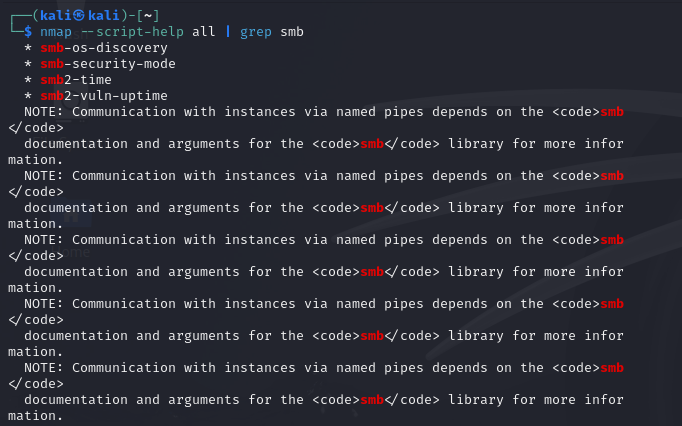
\includegraphics[width=1\textwidth]{Imagenes/ejercicio6.png}
         \caption{scripts SMB }
         \label{fig:eje6sc}
    \end{figure}

Entre todos los scripts, se utiliza específicamente aquellos relacionados con vulnerabilidades. Se especifica el asterisco para abarcar todos los scripts de vulnerabilidades SMB (\texttt{smb-vuln* }). Estos scripts son: \texttt{smb-vuln-ms10-061} (Identifica una vulnerabilidad en el servicio de impresión de Windows), \texttt{smb-vuln-ms17-010} (Detecta la vulnerabilidad EternalBlue) y \texttt{smb-vuln-ms10-054} (Detecta fallas en SMB que pueden ser explotadas). Además, para evitar escanear todos los puertos y reducir el tráfico de red, es recomendable especificar únicamente los puertos abiertos en la máquina objetivo.

    \begin{center}
    \texttt{nmap - -script=smb-vuln* 192.168.56.6 -p 80,135,139,445,49154,49156
    -oG ejercicio6W.txt}
    \end{center}
    

Al ejecutar el comando, se obtuvo información sobre el estado de los diferentes puertos y los resultados de 3 scripts de detección de vulnerabilidades en SMB. \\
En el caso del primero, se denegó el acceso, lo que significa que no se pudo verificar si la vulnerabilidad está presente. \\ 
Por otro lado, el script \texttt{smb-vuln-ms17-010} confirmó que el sistema es \textit{VULNERABLE} a MS17-010 (EternalBlue). Esta vulnerabilidad se identifica como \textt{CVE-2017-0143} y  significa que tiene una falla crítica en el protocolo SMBv1, permitiendo la ejecución remota de código sin autenticación. \\
Por último, el script \texttt{smb-vuln-ms10-054} dió como resutado \textit{False}, lo que indica que el sistema no es vulnerable a esa vulnerabilidad.
\newpage
    \begin{figure} [hp!]
         \centering
         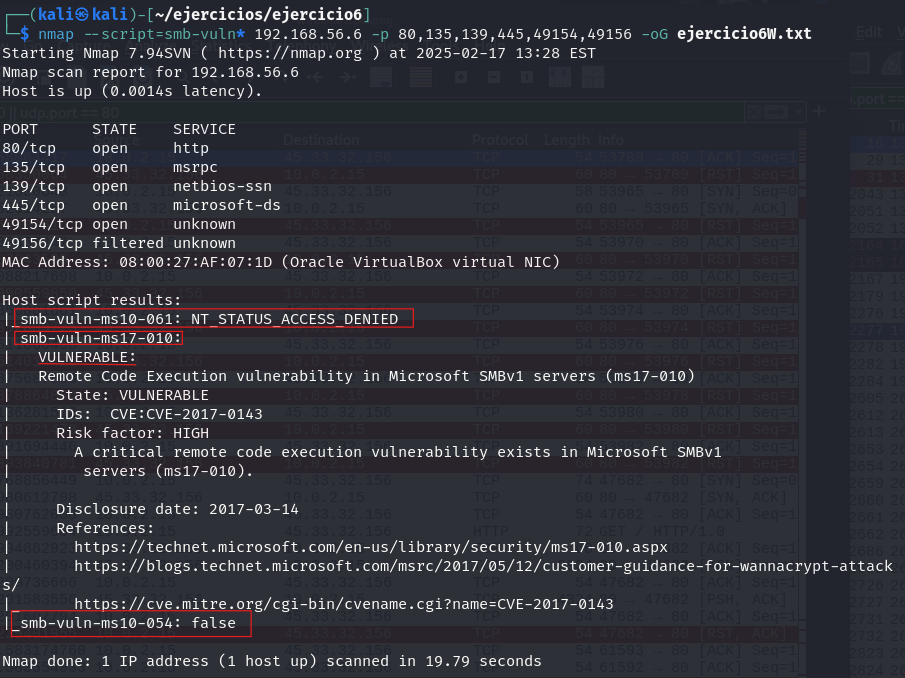
\includegraphics[width=1\textwidth]{Imagenes/eje6.png}
         \caption{scripts SMB - Máquina Windows}
         \label{fig:eje6}
    \end{figure}

De la misma manera, se ejecuta el escaneo en una máquina Linux, especificando solo los puertos abiertos para optimizar el análisis y realizar el mínimo ruido posible.

    \begin{center}
    \texttt{nmap - -script=smb-vuln* 192.168.56.9 -p
21,22,23,25,53,80,111,139,445,512,513,514,1099,1524,2049,2121,3306,5432,
5900,6000,6667,8009,8180 -oG ejercicio6L.txt}
    \end{center}

El resultado obtenido de los scripts, como se visualiza en la imagen \ref{fig:eje6Linuxm}, muestran que los scripts \texttt{smb-vuln-ms10-054} y \texttt{smb-vuln-ms10-061} son \textit{False}, lo que indica que no son vulnerables a esa vulnerabilidad. Mientras que en el caso del script \texttt{smb-vuln-regsvc-dos}, da un error en la ejecución. Para el último script, se recomienda utilizar la opción \texttt{-d} para realizar un debug. Esta opción hace que Nmap muestre mucha más información durante la ejecución, lo que hace que sea mucho más ruidosa. Como se tiene como objetivo realizar el menor ruido posible, y por tanto, menos tráfico y registros, es mejor no usar \texttt{-d}.
\newpage
    \begin{figure} [hp!]
         \centering
         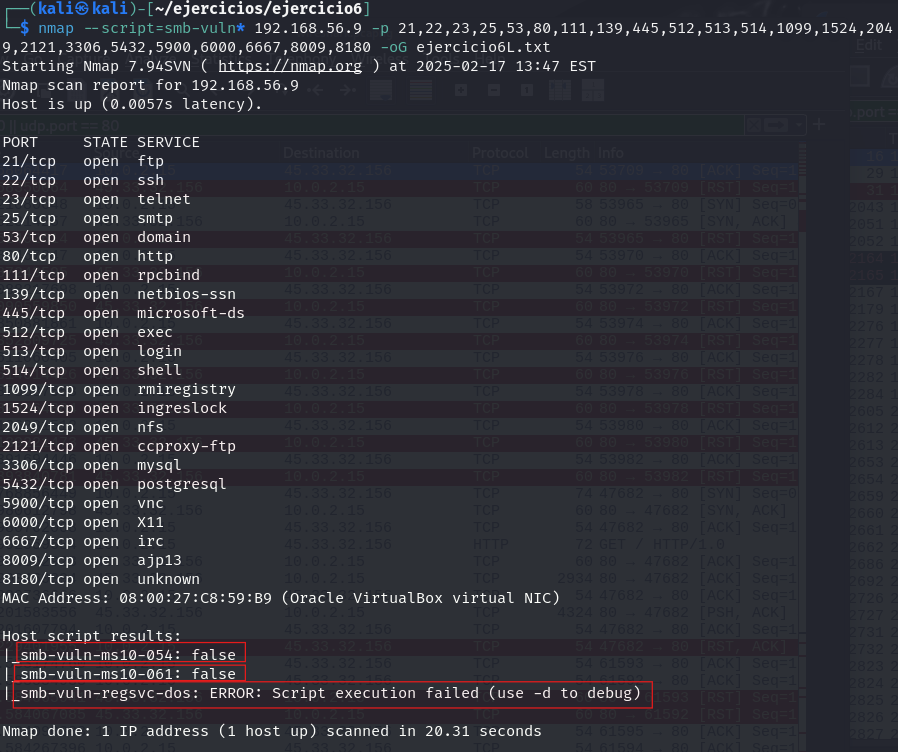
\includegraphics[width=1\textwidth]{Imagenes/eje6Linux.png}
         \caption{scripts SMB - Máquina Linux}
         \label{fig:eje6Linuxm}
    \end{figure}

    

\newpage
\\ \\
\section{Usando la funcionalidad NSE comprueba si el servicio http permite negociación de contenido.}
\\

En el caso de la máquina Windows, se especifican los puertos 80, 49154 y 49156. El puerto 80 ya que es el puerto estándar para HTTP. Mientras que los puertos 49154 y 49156,  aparecen como \texttt{unknown} en los resultados anteriores, lo que sugiere que podría estar siendo utilizado por alguna aplicación o servidor HTTP personalizado. 
\\ \\
    Dado que en la máquina Windows no hay un servidor Apache , el uso del script  \\ \texttt{http-apache-nonegotiation} no es el más adecuado para comprobar la negociación de contenido. Por lo que no existe un script NSE que, de manera precisa indique que un servidor HTTP está realizando negociación de contenido. En este caso, se utiliza el script \texttt{http-headers} para intentar obtener información sobre la respuesta HTTP. Sin embargo, no devuelve información relevante (cabeceras específicas) de negociación de contenido para esos puertos. El comando utilizado es: 
        \begin{center}
        \texttt{nmap - -script=http-headers 192.168.56.6 -p 80,49154,49156 -oG ejercicio76.txt}
        \end{center}

        
        \begin{figure} [hp!]
         \centering
         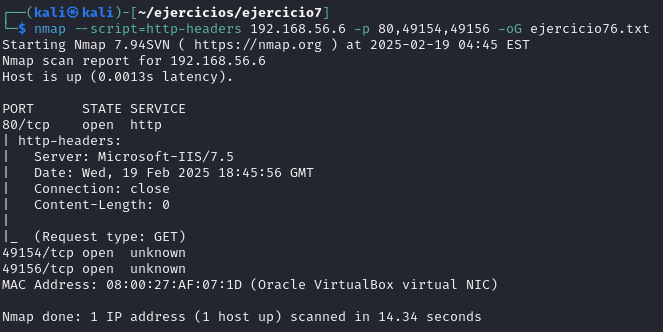
\includegraphics[width=1\textwidth]{Imagenes/httpheaders.png}
         \caption{script (http-headers) - Máquina Windows}
         \label{fig:eje6Linux}
        \end{figure}

Por otro lado, en la máquina de Linux si que hay servidor Apache, por lo que si que se utiliza el script \texttt{http-apache-nonegotiation}. Este script verifica si el servidor HTTP tiene habilitado el módulo \textit{mod\_negotiation} de Apache, que es responsable de la negociación de contenido. Además, se especifican los puertos 80 y 8180. El puerto 80 ya que es el puerto estándar para HTTP. Mientras, el puerto 8180 aparece como \texttt{unknown} en los resultados anteriores, lo que sugiere que podría estar siendo utilizado por alguna aplicación o servidor HTTP personalizado. El comando utilizado es:

    \begin{center}
    \texttt{nmap - -script=http-apache-negotiation 192.168.56.9 -p 80,8180 -oG ejercicio79.txt}
    \end{center}

    En este caso, el puerto 80/tcp está abierto y el script indica que el módulo \textit{mod\_negotiation} está habilitado, lo que significa que el servidor HTTP está configurado para permitir la negociación de contenido. 

        \begin{figure} [hp!]
         \centering
         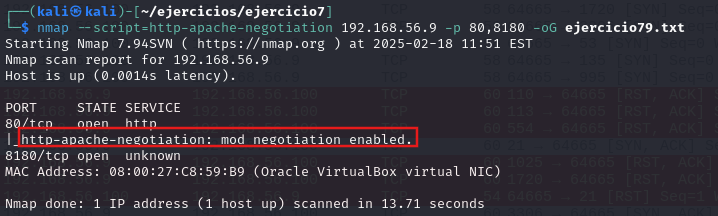
\includegraphics[width=1\textwidth]{Imagenes/eje7L.png}
         \caption{script (http-apache-negotiation) - Máquina Linux}
         \label{fig:eje6Linux}
        \end{figure}
        
\section{Referencias}
\printbibliography[heading=none]
\end{document}